\documentclass{article}

\usepackage[english]{babel}
\usepackage{microtype}
\usepackage{graphicx}
\usepackage{wrapfig}
\usepackage{enumitem}
\usepackage{fancyhdr}
\usepackage{amsmath}
\usepackage{chemformula}
\usepackage{index}
\usepackage{hyperref}
\usepackage[margin=1.0in]{geometry}
\usepackage{qtree}
\usepackage{float}
\usepackage{booktabs}
\usepackage{tabularx}
\usepackage{textcomp}

\begin{document}
\title{Summary: Reproduction and Embryonic Development}
\author{Dowland Aiello}
\date{April 9, 2020}

\maketitle
\tableofcontents
\fancyhf{}

\newpage

\section{The nature of asexual reproduction}

\textbf{Reproduction}, or ``the creation of new individuals from existing ones''
is essential to the continuation of life over the lifespan of an organism.
\textbf{Asexual reproduction} is one permutation of the two types of reproduction:
sexual reproduction and asexual reproduction. In contrast to \emph{sexual} reproduction,
\emph{asexual} reproduction poses no stipulations as to genetic diversity, nor
the ability of a parent organism to find a mate: an organism may reproduce without
sex via budding, fission, or the process of fragmentation and regeneration, for
example.

\bigbreak{}

\begin{table}[h]
	\begin{tabularx}{\linewidth}{>{\parskip1ex}X@{\kern4\tabcolsep}>{\parskip1ex}X}
	\toprule
	\hfil\bfseries Advantages
	&
	\hfil\bfseries Disadvantages
	\\\cmidrule(r{3\tabcolsep}){1-1}\cmidrule(l{-\tabcolsep}){2-2}

	%% PROS
	Allows animals that live in isolation to produce offspring\par
	Perpetuates a particular genotype precisely and rapidly\par

	&

	%% CONS
	Produces genetically uniform populations\par

	\\\bottomrule
	\end{tabularx}
	\caption{Advantages and disadvantages associated with asexual reproduction}
\end{table}

\section{The nature of sexual reproduction}

\textbf{Sexual reproduction}, or ``the creation of genetically unique offspring
by the fusion of two haploid sex cells (gametes), orming a diploid zygote'' is
an alternative pathway to ``reproduction'' in organisms where the
\textbf{fertilization} of \textbf{gamete} cells---sex cells with \emph{n}
chromosomes---is the desired mode of reproduction.
In organisms where the mode of reproduction involves such fertilization, there
exist two types of gametes:

\begin{itemize}
	\item \textbf{Sperm}, the male gamete: travels by means of a flagellum

		and the

	\item \textbf{Egg}, the female gamete: is not self-propelled
\end{itemize}

The fusion of the two aforementioned cells leads to the formation of a
\textbf{zygote}, which develops into a new individual.

In contrast with asexual reproduction, sexual reproduction increases genetic
diversity in the resulting population through random fertilization and
meiosis. The combination of these randomization factors results in the
principal force of natural selection: genetic variability.

\begin{wrapfigure}{r}{0.35\textwidth}
	\centering
	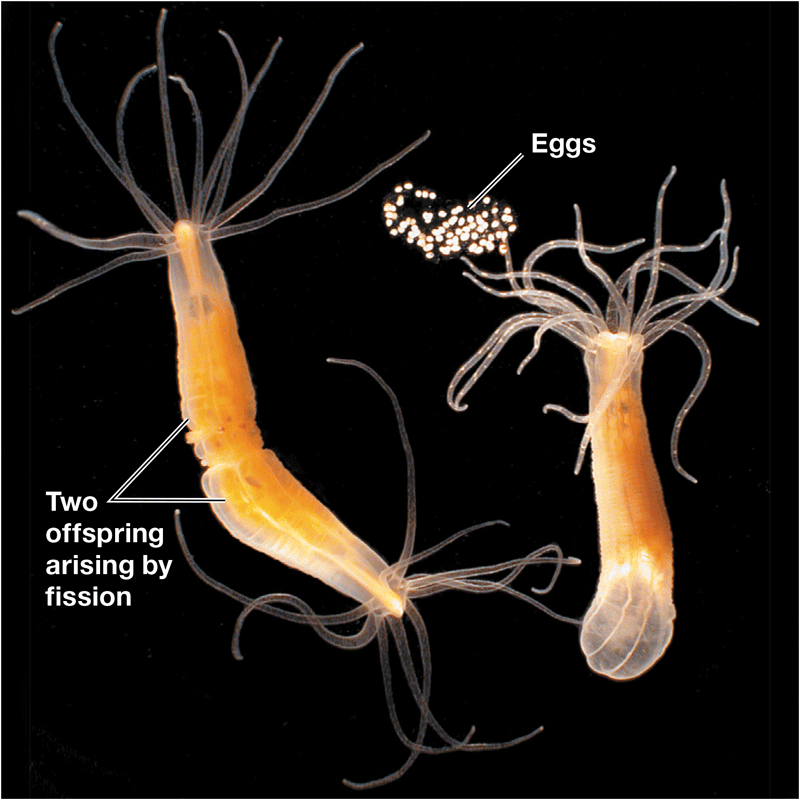
\includegraphics[width=0.9\linewidth]{hermaphroditism.png}
	\caption{The utilization of both asexual and sexual reproduction in the hydra.}
\end{wrapfigure}

While the aspect of variability associated with sexual reproduction might be
attractive for various mobile species, for isolated or immobile organisms,
sexual reproduction is implausible, as it requires a mate with which to
procreate. This inconvenience is addressed by the development of
\textbf{hermaphroditism}, or the existence of both female and male
reproductive systems in a single organism---``perfect'' flowers with both
stamens and carpels, are an example of such a development. The development
of hermaphroditism can be seen as advantageous, as it allows for animals to
reproduce with respect to environmental conditions.

\subsection{Different mechanisms for sexual reproduction}

Even with respect to sexual reproduction, there exist two separate development
of reproductive mechanisms:

\begin{itemize}
	\item \textbf{Reproduction by external fertilization}: gametes are released
		into and fuse in the environment---this is common in various acquatic animals
	\item \textbf{Reproduction by internal fertilization}: sperm are depsoited
		in or near the female reproductive tract
\end{itemize}

\section{The human female reproductive system}

\begin{wrapfigure}{l}{0.5\textwidth}
	\centering
	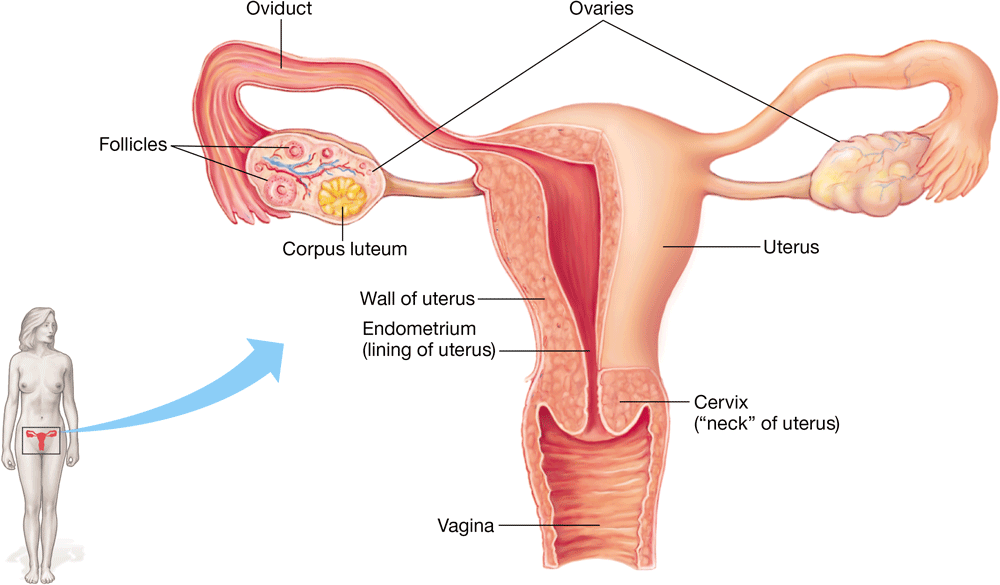
\includegraphics[width=0.9\linewidth]{female_reproductive_system.png}
	\caption{A diagram of the female human reproductive system.}
\end{wrapfigure}

The \textbf{ovaries} are the gamete-producing organs in the female reproductive
system, and can be described as having a ``bumpy'' surface---caused by the
\textbf{follicles} that both produce estrogen and enclose a developing egg cell.

In the process of \textbf{ovulation}, a female will release an immature egg via the
cilia lining the \textbf{oviduct}, or \emph{fallopian tube}---
after starting puberty, of course---as a result of the maturation of a follicle,
every 28 days. In addition, after having matured and formed the \textbf{corpus luteum},
a follicle will begin to release progestrone, alongside additional estrogen, complementing
the maintainence of the uterine lining. This process usually ceases near the age of 50.

With consideration to the above structural definitions, the following statements
regarding the development of a zygote, and the eventual birth of a human fetus
can be made:

\begin{enumerate}
	\item When ovulation occurs, if sperm are present in the upper part of the oviduct,
		fertilization may occur.
	\item After fertilization occurs, the zygote should continuously divide as it traverses
		the oviduct, eventually becoming an embryo.
	\item In the \textbf{uterus}---the site of
		pregnancy\footnote{In rare cases, an \textbf{ectopic pregnancy} may
		commence, where an embryo implants itself in the oviduct, potentially
		rupturing surrounding tissues.}---, an \textbf{embryo} will be
		deposited in the inner lining of the uterus \textbf{endometrium}.
	\item After implantation, the embryo will complete development until the 8th week of
		pregnancy, when the developing human will, henceforth, be referred to as a
		\textbf{fetus}.
	\item After continued development of the fetus, the \textbf{vagina} will serve as the
		canal through which the baby is born. The vagina is separated from the uterus by
		the \textbf{cervix}---the ``neck'' of the uterus.
\end{enumerate}

In addition to each of the aforementioned structures utilized in embryonic and
fetal development, various external structures collectively referred to as the
\textbf{vulva} provide functionality in
copulation\footnote{The \textbf{hymen} could be categorized as one such structure,
but provides little functionality in reproduction, and is ruptured in vigorous
physical activity or intercourse.}:

\begin{itemize}
	\item In sexual intercourse, the \textbf{vagina} serves as a repository for sperm, and
		is guarded by the \textbf{labia minora} and \textbf{labia majora}.
	\item Though it does not provide additional \emph{necessary} functionality in
		reproduction, the \textbf{clitoris}---an erectile organ consisting of a short shaft,
		followed by the \textbf{prepuce}, a small hood of highly sensitive skin---does serve
		a purpose in reproduction in that it evokes a highly presurable sensation when
		stimulated. As do the vagina and th elabia minor, this organ enlarges during sexual
		activity as a result of increased concentration of blood in the area.
\end{itemize}

\section{The human male reproductive system}

As is the case with many other mammals, the natural temperature of the human body presents a
challenge for the proper development of sperm cells within the \textbf{testes}---the male
gonads. That is, in humans, the most desirable temperature for sperm development is
approximately 2\textdegree{C} less than the normal human body temperature of
36.5--37.5\textdegree{C}. In humans, the \textbf{scrotum} solves this dilemma by keeping
sperm-forming cells within the acceptable temperature range.

After a sufficient volume of sperm cells have been produced in the testes, sperm leave
the gonads through the \textbf{epididymis}, where sperm cells will continue to develop
until \textbf{ejaculation}.

\end{document}
